\documentclass{ximera}

\begin{document}
	\author{Stitz-Zeager}
	\xmtitle{Exercises for Rational Inequalities}{}

\mfpicnumber{1} \opengraphsfile{ExercisesforRationalIneq} % mfpic settings added 

\begin{question}
(Review of Solving Equations):\footnote{For more review, see Section \ref{AppRatExpEqus}.} 

In Exercises \ref{ratleqnexercisefirst} - \ref{ratleqnexerciselast},  solve the rational equation.  Be sure to check for extraneous solutions.

\begin{problem}\label{ratleqnexercisefirst}
$\dfrac{x}{5x + 4} = 3$ 

\begin{solution}
$x = -\frac{6}{7}$
\end{solution}
\end{problem}

\begin{problem}
$\dfrac{3x - 1}{x^{2} + 1} = 1$ 
\end{problem} 

\begin{problem}
$\dfrac{1}{t + 3} + \dfrac{1}{t - 3} = \dfrac{t^{2} - 3}{t^{2} - 9}$ 

\begin{solution}
$t = -1$
\end{solution}
\end{problem} 

\begin{problem}
$\dfrac{2t + 17}{t + 1} = t + 5$ 
\end{problem}  

\begin{problem}
$\dfrac{z^{2} - 2z + 1}{z^{3} + z^{2} - 2z} = 1$ 

\begin{solution}
No solution
\end{solution}
\end{problem}   

\begin{problem}\label{ratleqnexerciselast}
$\dfrac{4z- z^3}{z^{2} - 9} = 4z$  
\end{problem}  

\end{question}

\begin{question}
In Exercises \ref{ratlineqexercisefirst} - \ref{ratlineqexerciselast}, solve the rational inequality.  Express your answer using interval notation.


\begin{problem}\label{ratlineqexercisefirst}
$\dfrac{1}{x + 2} \geq 0$ 

For what value of the domain is the rational function undefined? $\answer{-2}$
\begin{problem}
Use test points to determine all intervals which are part of the solution set.
    \begin{selectAll}
    \choice{$(-\infty,-2)$} \choice[correct]{$(-2,\infty)$}
  \end{selectAll}
\end{problem}
\end{problem} 

\begin{problem}
$\dfrac{5}{x + 2} \geq 1$
\end{problem} 

\begin{problem}
$\dfrac{x}{x^{2} - 1} <  0$

For which values is the rational function undefined? $\answer{0}$

For which values is the rational function undefined? (Give your answers in increasing order.) $\answer{-1}$ $\answer{1}$

\begin{problem}
Use test points to determine all intervals which are part of the solution set.
    \begin{selectAll}
    \choice[correct]{$(-\infty,-1)$} 
    \choice{$(-1,0)$}
    \choice[correct]{$(0,1)$} 
    \choice{$(1,\infty)$}
  \end{selectAll}
\end{problem}
\end{problem}  

\begin{problem}
$\dfrac{4t}{t^2+4} \geq 0$
\end{problem}    

\begin{problem}
$\dfrac{2t+6}{t^2+t-6} < 1$
\end{problem}

\begin{problem}
$\dfrac{5}{t-3} + 9 < \dfrac{20}{t+3}$
\end{problem}

\begin{problem}
$\dfrac{6z+6}{2+z-z^2} \leq z+3$
\end{problem}  

\begin{problem}
$\dfrac{6}{z-1} + 1 > \dfrac{1}{z+1}$
\end{problem}  

\begin{problem}
$\dfrac{3z - 1}{z^{2} + 1} \leq 1$
\end{problem}

\begin{problem}
$(2x+17)(x+1)^{-1} > x + 5$
\end{problem} 

\begin{problem}
$(4x-x^3)(x^{2} - 9)^{-1} \geq 4x$
\end{problem} 

\begin{problem}
$(x^{2} + 1)^{-1} < 0$
\end{problem}  

\begin{problem}
$(2t-8)(t+1)^{-1} \leq (t^2-8t)(t+1)^{-2}$ % $[-4, -1) \cup (-1,2]$
\end{problem}  

\begin{problem}
$(t-3)(2t+7)(t^2+7t+6)^{-2} \geq (t^2+7t+6)^{-1}$ % $(-\infty, -6) \cup (-6, -3] \cup [9, \infty)$
\end{problem} 

\begin{problem}
$60z^{-2}+23z^{-1} \geq 7(z-4)^{-1}$
\end{problem} 

\begin{problem}\label{ratlineqexerciselast}
$2z+6(z-1)^{-1} \geq 11 - 8(z+1)^{-1}$
\end{problem}  
\end{question}

\begin{question}
In Exercises \ref{solverationalineqfromgraphfirst} - \ref{solverationalineqfromgraphlast}, use the the graph of the given rational function to  solve the stated inequality.    

\begin{problem}\label{solverationalineqfromgraphfirst}
Solve $f(x) \geq 0$.


\begin{tikzpicture}
  \begin{axis}[
    axis lines=middle,
    xmin=-7, xmax=7,
    ymin=-6, ymax=8,
    xtick={-6,-5,-4,-3,-2,-1,1,5,6},
    xticklabels={$-6$,$-5$,$-4$,$-3$,$-2$,$-1$,$1$,$5$,$6$},
    ytick={-5,-4,-3,-2,-1,1,2,3,4},
    yticklabels={$-5$,$-4$,$-3$,$-2$,$-1$,$1$,$2$,$3$,$4$},
    axis line style={->},
    width=11cm, height=8cm,
    clip=false
  ]
    % Axis labels
    \node at (axis cs:7,-0.5) {\scriptsize $x$};
    \node at (axis cs:0.5,8) {\scriptsize $y$};

    % Horizontal asymptote y=1
    \draw[dashed] (axis cs:-7,1) -- (axis cs:7,1);

    % Vertical asymptote x=0
    \draw[dashed] (axis cs:0,-6) -- (axis cs:0,8);

    % Function y = 1 - 3/x
    \addplot[domain=-7:-0.45, samples=200, thick, ->] {1 - 3/x};
    \addplot[domain=0.45:7, samples=200, thick, ->] {1 - 3/x};

    % Point (3,0)
    \addplot[only marks, mark=*] coordinates {(3,0)};
    \node at (axis cs:3.5,-1) {\scriptsize $(3,0)$};

    % Caption
    \node[below] at (rel axis cs:0.5,0) 
      {\scriptsize $y=f(x)$, asymptotes: $x=0$, $y=1$};
  \end{axis}
\end{tikzpicture}

\end{problem}

\begin{problem}
Solve $f(x) < 1$.


\begin{tikzpicture}
  \begin{axis}[
    axis lines=middle,
    xmin=-7, xmax=7,
    ymin=-6, ymax=8,
    xtick={-6,-5,-4,-3,-2,-1,1,5,6},
    xticklabels={$-6$,$-5$,$-4$,$-3$,$-2$,$-1$,$1$,$5$,$6$},
    ytick={-5,-4,-3,-2,-1,1,2,3,4},
    yticklabels={$-5$,$-4$,$-3$,$-2$,$-1$,$1$,$2$,$3$,$4$},
    axis line style={->},
    width=11cm, height=8cm,
    clip=false
  ]
    % Axis labels
    \node at (axis cs:7,-0.5) {\scriptsize $x$};
    \node at (axis cs:0.5,8) {\scriptsize $y$};

    % Horizontal asymptote y=1
    \draw[dashed] (axis cs:-7,1) -- (axis cs:7,1);

    % Vertical asymptote x=0
    \draw[dashed] (axis cs:0,-6) -- (axis cs:0,8);

    % Function y = 1 - 3/x
    \addplot[domain=-7:-0.45, samples=200, thick, ->] {1 - 3/x};
    \addplot[domain=0.45:7, samples=200, thick, ->] {1 - 3/x};

    % Point (3,0)
    \addplot[only marks, mark=*] coordinates {(3,0)};
    \node at (axis cs:3.5,-1) {\scriptsize $(3,0)$};

    % Caption
    \node[below] at (rel axis cs:0.5,0) 
      {\scriptsize $y=f(x)$, asymptotes: $x=0$, $y=1$};
  \end{axis}
\end{tikzpicture}

\end{problem} 

\begin{problem}
Solve $g(t) \geq  -1 $. 

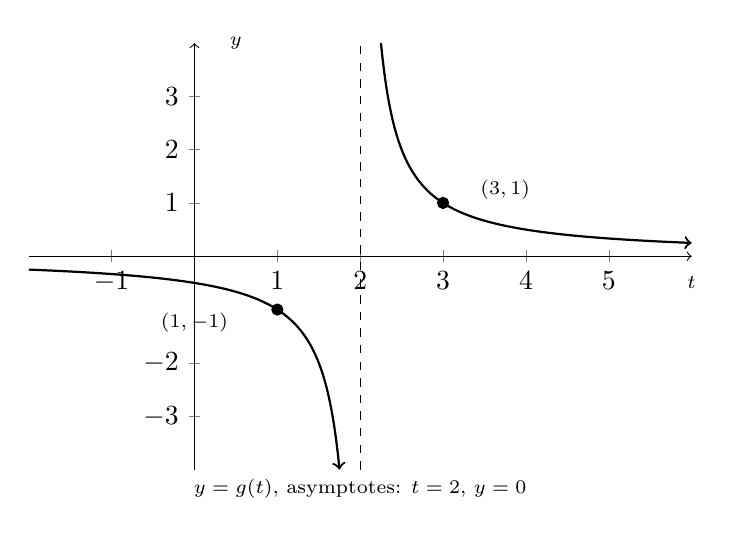
\begin{tikzpicture}
  \begin{axis}[
    axis lines=middle,
    xmin=-2, xmax=6,
    ymin=-4, ymax=4,
    xtick={-1,1,2,3,4,5},
    xticklabels={$-1$,$1$,$2$,$3$,$4$,$5$},
    ytick={-3,-2,1,2,3},
    yticklabels={$-3$,$-2$,$1$,$2$,$3$},
    axis line style={->},
    width=10cm, height=7cm,
    clip=false
  ]
    % Axis labels
    \node at (axis cs:6,-0.5) {\scriptsize $t$};
    \node at (axis cs:0.5,4) {\scriptsize $y$};

    % Vertical asymptote t=2
    \draw[dashed] (axis cs:2,-4) -- (axis cs:2,4);

    % Horizontal asymptote y=0
    \draw[dashed] (axis cs:-2,0) -- (axis cs:6,0);

    % Function y = 1/(x-2)
    \addplot[domain=-2:1.75, samples=200, thick, ->] {1/(x-2)};
    \addplot[domain=2.25:6, samples=200, thick, ->] {1/(x-2)};

    % Solid points
    \addplot[only marks, mark=*] coordinates {(1,-1) (3,1)};
    \node at (axis cs:3.75,1.25) {\scriptsize $(3,1)$};
    \node at (axis cs:0,-1.25) {\scriptsize $(1,-1)$};

    % Caption
    \node[below] at (rel axis cs:0.5,0) 
      {\scriptsize $y=g(t)$, asymptotes: $t=2$, $y=0$};
  \end{axis}
\end{tikzpicture}

\end{problem}   

\begin{problem}
Solve $-1 \leq g(t)  < 1$. 

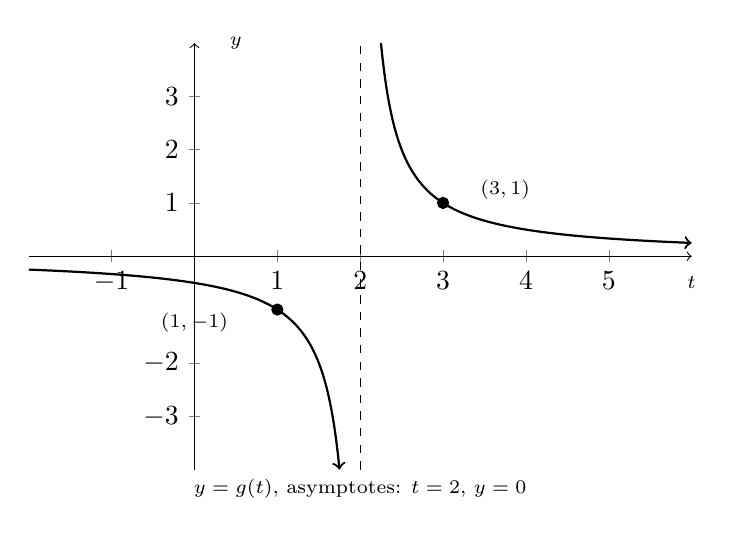
\begin{tikzpicture}
  \begin{axis}[
    axis lines=middle,
    xmin=-2, xmax=6,
    ymin=-4, ymax=4,
    xtick={-1,1,2,3,4,5},
    xticklabels={$-1$,$1$,$2$,$3$,$4$,$5$},
    ytick={-3,-2,1,2,3},
    yticklabels={$-3$,$-2$,$1$,$2$,$3$},
    axis line style={->},
    width=10cm, height=7cm,
    clip=false
  ]
    % Axis labels
    \node at (axis cs:6,-0.5) {\scriptsize $t$};
    \node at (axis cs:0.5,4) {\scriptsize $y$};

    % Vertical asymptote t=2
    \draw[dashed] (axis cs:2,-4) -- (axis cs:2,4);

    % Horizontal asymptote y=0
    \draw[dashed] (axis cs:-2,0) -- (axis cs:6,0);

    % Function y = 1/(x-2)
    \addplot[domain=-2:1.75, samples=200, thick, ->] {1/(x-2)};
    \addplot[domain=2.25:6, samples=200, thick, ->] {1/(x-2)};

    % Solid points
    \addplot[only marks, mark=*] coordinates {(1,-1) (3,1)};
    \node at (axis cs:3.75,1.25) {\scriptsize $(3,1)$};
    \node at (axis cs:0,-1.25) {\scriptsize $(1,-1)$};

    % Caption
    \node[below] at (rel axis cs:0.5,0) 
      {\scriptsize $y=g(t)$, asymptotes: $t=2$, $y=0$};
  \end{axis}
\end{tikzpicture}
\end{problem} 

\begin{problem}
Solve $r(z) \leq 1$ 

\begin{tikzpicture}
  \begin{axis}[
    axis lines=middle,
    xmin=-5, xmax=5,
    ymin=-1, ymax=6,
    xtick={-4,-3,-2,-1,1,2,3,4},
    xticklabels={$-4$,$-3$,$-2$,$-1$,$1$,$2$,$3$,$4$},
    ytick={1,2,3,4,5},
    yticklabels={$1$,$2$,$3$,$4$,$5$},
    axis line style={->},
    width=11cm, height=8cm,
    clip=false
  ]
    % Axis labels
    \node at (axis cs:5,-0.5) {\scriptsize $z$};
    \node at (axis cs:0.5,6) {\scriptsize $y$};

    % Vertical asymptote z=0
    \draw[dashed] (axis cs:0,-1) -- (axis cs:0,6);

    % Horizontal asymptote y=0
    \draw[dashed] (axis cs:-5,0) -- (axis cs:5,0);

    % Function y = 1/x^2
    \addplot[domain=-5:-0.42, samples=200, thick, ->] {1/(x^2)};
    \addplot[domain=0.42:5, samples=200, thick, ->] {1/(x^2)};

    % Solid point (-1,1)
    \addplot[only marks, mark=*] coordinates {(-1,1)};
    \node at (axis cs:-2.5,1) {\scriptsize $(-1,1)$};

    % Hole at (1,1)
    \addplot[only marks, mark=o, mark size=2pt, thick] coordinates {(1,1)};
    \node at (axis cs:3,1) {\scriptsize hole at $(1,1)$};

    % Caption
    \node[below] at (rel axis cs:0.5,0) 
      {\scriptsize $y=r(z)$, asymptotes: $z=0$, $y=0$};
  \end{axis}
\end{tikzpicture}


\end{problem} 

\begin{problem}\label{solverationalineqfromgraphlast} Solve $r(z) > 0$.


\begin{tikzpicture}
  \begin{axis}[
    axis lines=middle,
    xmin=-5, xmax=5,
    ymin=-1, ymax=6,
    xtick={-4,-3,-2,-1,1,2,3,4},
    xticklabels={$-4$,$-3$,$-2$,$-1$,$1$,$2$,$3$,$4$},
    ytick={1,2,3,4,5},
    yticklabels={$1$,$2$,$3$,$4$,$5$},
    axis line style={->},
    width=11cm, height=8cm,
    clip=false
  ]
    % Axis labels
    \node at (axis cs:5,-0.5) {\scriptsize $z$};
    \node at (axis cs:0.5,6) {\scriptsize $y$};

    % Vertical asymptote z=0
    \draw[dashed] (axis cs:0,-1) -- (axis cs:0,6);

    % Horizontal asymptote y=0
    \draw[dashed] (axis cs:-5,0) -- (axis cs:5,0);

    % Function y = 1/x^2
    \addplot[domain=-5:-0.42, samples=200, thick, ->] {1/(x^2)};
    \addplot[domain=0.42:5, samples=200, thick, ->] {1/(x^2)};

    % Solid point (-1,1)
    \addplot[only marks, mark=*] coordinates {(-1,1)};
    \node at (axis cs:-2.5,1) {\scriptsize $(-1,1)$};

    % Hole at (1,1)
    \addplot[only marks, mark=o, mark size=2pt, thick] coordinates {(1,1)};
    \node at (axis cs:3,1) {\scriptsize hole at $(1,1)$};

    % Caption
    \node[below] at (rel axis cs:0.5,0) 
      {\scriptsize $y=r(z)$, asymptotes: $z=0$, $y=0$};
  \end{axis}
\end{tikzpicture}


\end{problem} 

\end{question}


\begin{problem}
In Exercise \ref{newportaboycost} in Section \ref{GraphsofPolynomials},  the function $C(x) = .03x^{3} - 4.5x^{2} + 225x + 250$, for $x \geq 0$ was used to model the cost (in dollars) to produce $x$ PortaBoy game systems. Using this cost function, find the number of PortaBoys which should be produced to minimize the average cost $\overline{C}$.  Round your answer to the nearest number of systems.     
\end{problem}  

\begin{problem}
Suppose we are in the same situation as Example \ref{boxnotopfixedvolume}.  If the volume of the box is to be $500$ cubic centimeters, use a graphing utility to find the dimensions of the box which minimize the surface area.  What is the minimum surface area?  Round your answers to two decimal places.
\end{problem} 

\begin{problem}
The box for the new Sasquatch-themed cereal, `Crypt-Os', is to have a volume of $140$ cubic inches.  For aesthetic reasons, the height of the box needs to be $1.62$ times the width of the base of the box.\footnote{1.62 is a crude approximation of the so-called `Golden Ratio' $\phi = \frac{1 + \sqrt{5}}{2}$.}  Find the dimensions of the box which will minimize the surface area of the box.  What is the minimum surface area?  Round your answers to two decimal places.   
\end{problem}   

\begin{problem}\label{fixedareaminperimetergarden} 
Sally is Skippy's neighbor from Exercise \ref{fixedperimetermaxareagarden} in Section \ref{QuadraticFunctions}.   Sally also wants to plant a vegetable garden along the side of her home.  She doesn't have any fencing, but wants to keep the size of the garden to 100 square feet.  What are the dimensions of the garden which will minimize the amount of fencing she needs to buy?  What is the minimum amount of fencing she needs to buy? Round your answers to the nearest foot. (Note:  Since one side of the garden will border the house, Sally doesn't need fencing along that side.)
\end{problem}

\begin{problem}
Another Classic Problem: A can is made in the shape of a right circular cylinder and is to hold one pint. (For dry goods, one pint is equal to $33.6$ cubic inches.)\footnote{According to \href{http://dictionary.reference.com/browse/pint}{\underline{www.dictionary.com}}, there are different values given for this conversion. We use $33.6 \text{in}^{3}$ for this problem.}  

\begin{enumerate}

\item Find an expression for the volume $V$ of the can in terms of the height $h$ and the base radius $r$.
\item Find an expression for the surface area $S$ of the can in terms of the height $h$ and the base radius $r$.  (Hint: The top and bottom of the can are circles of radius $r$ and the side of the can is really just a rectangle that has been bent into a cylinder.)
\item Using the fact that $V = 33.6$, write $S$ as a function of $r$ and state its applied domain.
\item Use your graphing calculator to find the dimensions of the can which has minimal surface area.

\end{enumerate}
\end{problem}

\begin{problem}
A right cylindrical drum is to hold 7.35 cubic feet of liquid.  Find the dimensions (radius of the base and height) of the drum which would minimize the surface area.  What is the minimum surface area?  Round your answers to two decimal places.
\end{problem} 

\begin{problem}
In Exercise \ref{squatchpop} in Section \ref{IntroRational}, the population of Sasquatch in Portage County is modeled by  \[P(t) = \frac{150t}{t + 15}, \quad t \geq 0,\] where $t = 0$ corresponds to the year 1803.  According to this model, when were there fewer than 100 Sasquatch in Portage County?
\end{problem}




\end{document}
